\documentclass[12pt, a4paper,twoside]{tesi_upf}

%CODIFICACIÓ
\usepackage[utf8]{inputenc}
\usepackage{amssymb,amsmath}

\usepackage{url}

%IDIOMES
\usepackage[catalan,english]{babel}

%NOMÉS PER A OBTENIR INDICACIÓ DEL MARC EN MIDA A4
%\usepackage[cam,a4,center,frame]{crop}

\usepackage[toc,page]{appendix}

%PER A INCLOURE GRÀFICS I EL LOGO DE LA UPF
\usepackage{graphicx}

\usepackage[autostyle]{csquotes}
\usepackage{breakcites}
\usepackage{quotchap}

%PER CODI FONT
%\usepackage{listings}
\usepackage{caption}
\DeclareCaptionType{mycapequ}[][List of equations]
\captionsetup[mycapequ]{labelformat=empty}
%\captionsetup[lstlisting]{font={small,tt}}

%\usepackage{hyperref}

\usepackage[section]{placeins}

%FONTS TIMES O GARAMOND,
\usepackage{times}
%\usepackage{garamond}

%SENSE HEADINGS: NO MODIFICAR
\pagestyle{plain}

%PER A L'ÍNDEX DE MATÈRIES
%\usepackage{makeidx}
%\makeindex

%ESTIL DE BIBLIOGRAFIA
\bibliographystyle{apalike}

\renewcommand\appendixpage{}


%AQUEST DOCUMENT ÉS EN CATALÀ
\selectlanguage{english}

%EN COMPTES DE ÍNDEX, LA TAULA DE CONTINGUTS ES TITULA SUMARI
\addto\captionscatalan
  {\renewcommand{\contentsname}{\Large \sffamily Table of contents}}

\newcommand{\keyword}[1]{\textit{#1}}

%AFEGIU EN AQUESTA PART LES VOSTRES DADES
\title{Nucleo-olivary inhibition explains extinction on a computational model of the vestibulo-ocular reflex}
\author{Xavier Duran Albareda}
\thyear{2015}
\department{Synthetic Perceptive, Emotive and Cognitive Systems (SPECS)}
\supervisor{Dr. Ivan Herreros}
\director{Prof. Dr. Paul F.M.J Verschure}

\begin{document}


\frontmatter

\maketitle

\cleardoublepage


%%% Dedicatòria; si no es vol posar, comenteu fins a final de dedicatòria
\noindent Your hemoglobin molecules, your antibodies, your neurons, your vestibulo-ocular reflex machinery\textemdash at every level of analysis we find machinery that dumbly does a wonderful, elegantly designed job.
\cleardoublepage
%%% Final de dedicatòria

%%% Agraïments; si no es vol posar, comenteu fins a final de agraïments
\noindent {\Large \sffamily Acknowledgements}
\newline

I want to acknowledge my thesis supervisor, Ivan Herreros for his guidance and support during this project, Paul Verschure, Armin Duff, Riccardo Zucca and Anna Mura for their inspiring lectures and all the CSIMers for this shared experience.

\cleardoublepage
%%% Final dels agraïments

\vspace*{\fill}
\section*{\Large \sffamily Abstract}

Vestibulo-ocular reflex (VOR) adaptation is one of the most studied cerebellar dependent motor learning tasks. It is used to provide insight about the connections and the coding of the circuitry of the cerebellum. The state of the art computational models of the VOR don't define accurately the extinction of the reflex, that is modeled in the dark as in-phase with the vestibular information when no evidences have shown. This predicts a linear decay of the adaptation gain of the reflex, when an exponential decay has shown experimentally.

This study shows that nucleo-olivary inhibition (NOI) gives a more parsimonious explanation for the extinction of the acquired adaptation in VOR, exponential decay to the baseline gain.


Extinction is triggered when vestibular information is available
Teaching or error signal is modulated by cerebellar output
Savings

Classical models used to explain motor learning with a single site of plasticity on the cerebellar cortex, but on the last decade a growing body of evidence has shown that plasticity on the brainstem is also needed for the adaptation.


\vskip 1cm

Keywords: \keyword{vestibulo-ocular reflex}, \keyword{cerebellum}, \keyword{nucleo-olivary inhibition}, \keyword{extinction}, \keyword{reflex}

\vspace*{\fill}

\cleardoublepage
%FIN DE ABSTRACTE

%PREFACI OPCIONAL. SI NO ES VOL, COMENTEU FINS EL FINAL DE PREFACI
%{\bf Prefaci}
\cleardoublepage
%FINAL DE PREFACI

%TAULA DE CONTINGUTS: OBLIGATÒRIA
\tableofcontents

%INDEX DE FIGURES; NOMÉS ES POSA SI HI HA FIGURES
\listoffigures
%Fa que aparegui al sumari
\addcontentsline{toc}{chapter}{Índex de figures}

%INDEX DE TAULES; NOMÉS ES POSA SI HI HA TAULES
%\listoftables
%Fa que aparegui al sumari
%\addcontentsline{toc}{chapter}{Índex de taules}

\mainmatter
\chapter{Introduction}

\section{Problem statement}

Vestibulo-ocular reflex (VOR) is one of the most studied cerebellar dependent motor learning tasks, and its study is used to provide insight about the connections and the coding of the circuitry of the cerebellum. The funcion of the VOR is to stabilize the images on the retina during head movement by producing eye movements in the opposite direction to that head movement. Thanks to this reflex, the image remains on the center of the visual field.

VOR is naturally adapted during lifetime due to multiple reasons. Growth, changes in the body or wearing glasses are among them and may cause variations on the parameters of the reflex to adapt to the new situation.

When the adaptation is no longer needed, there is an extinction of the reflex. The mechanisms of this extinction are poorly understood and have not been suitably described on computational models of the VOR. The problem is that state of the art computational models of the vestibulo-ocular reflex don't define an existing physiological mechanism for extinction. Instead of this, they try to reproduce the behavior of the reflex by introducing artificial extinction mechanisms.

This study gives a more parsimonious explanation of the extinction phenomena by means of the nucleo-olivary inhibition (NOI), a physiological connection that has been shown to work as an extinction of the adaptation on eye-blink reflex conditioning  \cite{Emken2007, Herreros2013b}, a reflex whose cerebellar circuitry is very similar to VOR's.

\section{State of the art}

The cerebellum has a central role in motor learning, that is the process of improving the smoothness and accuracy of movements through practice. It is not only important for learning to perform complicated movements, like playing an instrument or a sport, but also for adaptation of simple movements like reflexes along the physical changes that may occur over time. This role was early discovered studying patients with ataxia, a sensori-motor syndrome related to cerebellar malfunction and diseases \cite{Mapelli2015}.

The cerebellar cortex seems to have a uniform structure throughout the cerebellum. Its architecture is sometimes described as crystalline for it appears to be an homogeneous sheet of tissue, and is composed of repeated modules or microzones, that have the same cell types that are connected in the same manner and are the functional units of the cerebellar cortex. Depending on its functional role, different microzones receive different inputs and project to different targets. A microzone along with its related subcortical structures forms what's called a microcomplex \cite{Ito1982}, and it's considered to be a unit neuronal machine.

The uniformity on the microcircuit of the cerebellar cortex has inspired the idea that there is a single cerebellar algorithm and that different microzones process signals they receive in a similar way. The study of the cerebellum during one specific learning task may help to generalize its function to be applied to many different tasks \cite{Boyden2004}.

The flocculus, a small lobe situated on the vestibulocerebellum, is the main cerebellar region that is responsible of the control of eye movements. Its role is to optimize ocular motor performance so that the image remains still enough on the fovea so the brain is able to interpret the scene in real time \cite{Kheradmand2011}. The flocculus receives visual and vestibular information and uses it to control gaze stabilization. Vestibulo-ocular reflex, optokinetic nystagmus and smooth pursuit are under the control of the floccular region of the cerebellum.

\subsection{Vestibulo-ocular reflex (VOR)}

VOR is a compensatory eye movement that stabilizes retinal images during head movements by producing an eye movement in the opposite direction, thus preventing degradation of image processing. During lifetime, changes in vestibular processing or in the mechanical properties of the oculomotor plant (as muscles develop or weaken) can cause eye-movement inaccuracies. This poor calibration results in blurred vision and VOR needs to be adapted, and the same happens when a subject starts to wear glasses. VOR produces compensatory movements in response to horizontal, vertical and translational head movements (Figure \ref {fig:vor}).

\begin{figure}
  \centering
  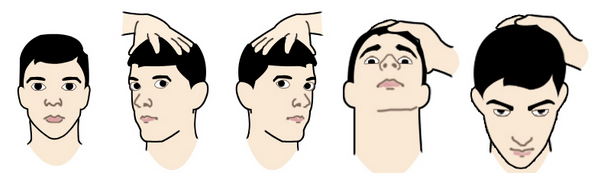
\includegraphics[scale=0.70]{images/vor.png}
  \caption[VOR reflex]{VOR reflex}
  \label{fig:vor}
\end{figure}

The cerebellar cortex receives two differents sensory signals: head movement or vestibular information and retinal slip or visual information \cite{Boyden2004}, and outputs a motor command to generate the compensatory eye movements (Figure \ref {fig:vorboyden}).

\begin{figure}
  \centering
  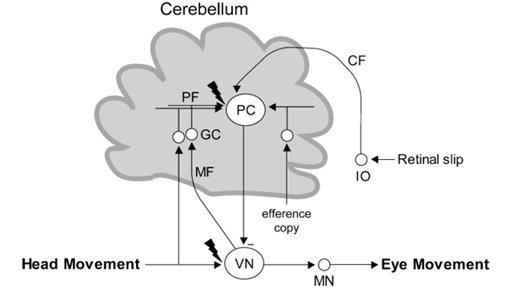
\includegraphics[scale=0.70]{images/boyden.png}
  \caption[Simplified schema of VOR reflex circuitry on the cerebellum]{Simplified schema of VOR reflex circuitry on the cerebellum}
  \label{fig:vorboyden}
\end{figure}

In terms of control theory, VOR is a feedforward or open-loop control system since the output of the reflex has no effect on the vestibular signals input \cite{Porrill2007}, and it's controlled by an adaptive mechanism of the cerebellum. This adaptation is materialized by changing the amplitude and timing of the VOR, expressed in gain and phase values respectively \cite{DeZeeuw2005}.

\subsubsection{VOR adaptation}

In the laboratory VOR adaptation is induced in training sessions by providing visual stimuli in conflict with the vestibular stimulus. Typically screen and turntable rotation are combined to induce bidirectional gain changes in the animal VOR. Depending on the relative direction of the head and the image motion, gain and phase parameters can increase or decrease after the training periods.

\begin{figure}
  \centering
  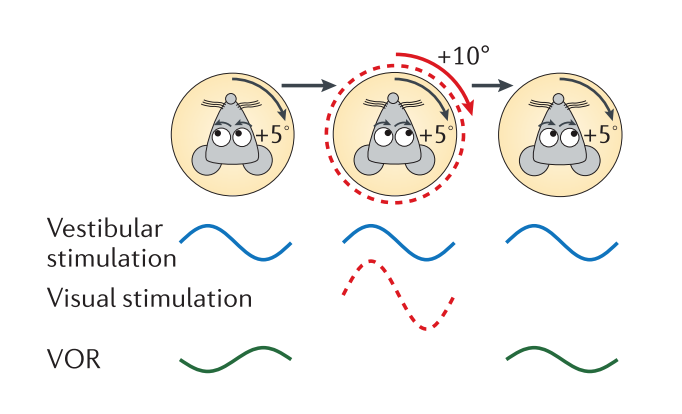
\includegraphics[scale=0.50]{images/vor_adaptation.png}
  \caption[VOR reflex phase reversal adaptation protocol]{VOR reflex phase reversal adaptation protocol \cite{Gao2012a}}
  \label{fig:voradaptation}
\end{figure}

An image motion in the opposite direction as the head induces gain increase while the image in the same direction induces gain decrease. In gain-decrease learning, VOR cancellation happens when the speed of the head and the image are the same, and phase-reversal learning when the image is faster (Figure \ref {fig:voradaptation}).

After training sessions, the performance of the VOR is measured in the dark to isolate the eye response due to head movements from that driven by visual stimuli. The persistence of the changes depends on the length of the training and the history of eye movement. VOR adaptation is trained with light and measured in the dark \cite{Boyden2004}.

The flocculus or the entire cerebellum is not critical for generating the VOR, as it is still present in animals with the complete ablation of it, but it remains necessary for its adaptation. Lesions on the inferior olive also ended with the same result \cite{Ito2006}. This shows that the olivo-cerebellum is necessary for the adaptation of the reflex.

\subsection{Extinction of the learned adaptation}

Head movements in the absence of visual stimulation cause a loss of the learned eye movement response. This loss is measured by changes in the amplitude of the eye movements, defined as the gain of the VOR. When neither visual nor vestibular information is present, the gain of the VOR remains stable.

This means that the extinction of the learned adaptation is mediated by an active, extinction-like process and not by passive forgetting \cite{Cohen2004}.

\subsubsection{Nucleo-olivary inhibition (NOI): a candidate signal}

Nucleo-olivary inhibition is an inhibitory synaptic connection between a population of neurons on the cerebellar nuclei and the inferior olive. This connection causes the inhibition of the climbing fibres, the neurons that carry the retinal slip, and serves as a teaching signal for extinction \cite{Medina2002} on the inferior olive, so that the inactivation of the NOI prevents extinction.

On the eye-blink reflex adaptation paradigm, when the acquired conditioned response is no longer necessary, nucleo-olivary inhibition has been described to work as a cost minimization mechanism between the cost of the aversive stimuli and that of the unnecesary avoidance \cite{Brandi2013}, thus balancing the cost between adaptive and reactive reflexes.

Similarities between eye-blink conditioning (Figure \ref {fig:eyeblinkcircuitry}) and VOR reflex (Figure \ref {fig:vorcircuitry}) circuitry are well known. This fact suggests the possibility of NOI having an active role in extinction on VOR.

\begin{figure}
  \centering
  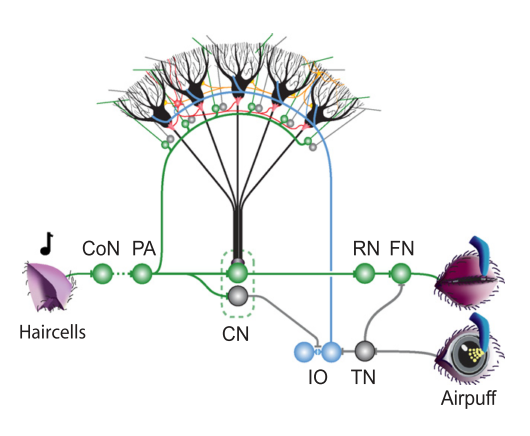
\includegraphics[scale=0.50]{images/schonewille-ebc.png}
  \caption[Neuroanatomical circuitry involved in eyeblink conditioning]{Neuroanatomical circuitry involved in eyeblink conditioning \cite{Schonewille2011}}
  \label{fig:eyeblinkcircuitry}
\end{figure}

\begin{figure}
  \centering
  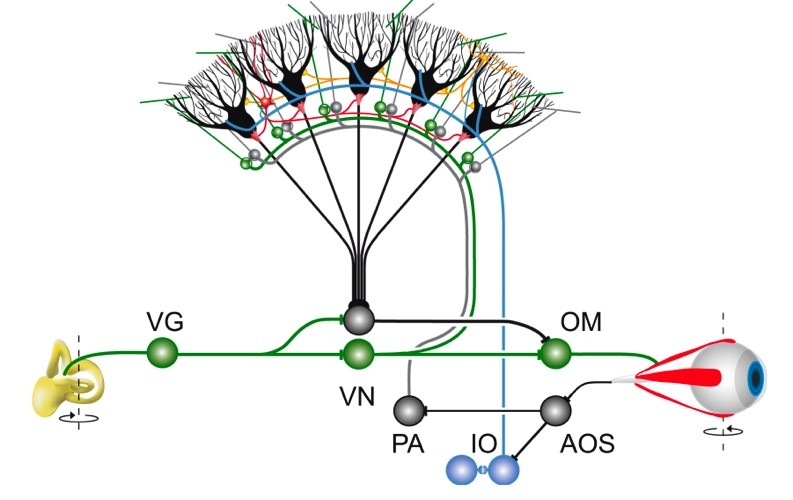
\includegraphics[scale=0.50]{images/schonewille.png}
  \caption[Neuroanatomical circuitry involved in VOR]{Neuroanatomical circuitry involved in VOR \cite{Schonewille2011}}
  \label{fig:vorcircuitry}
\end{figure}

\chapter{Methods}

\section{Research Question}

Would nucleo-olivary inhibition explain extinction in the vestibulo-ocular reflex computational models?

\subsubsection{In direct evidence}

There is extinction of the adaptive response in the absence of peripheral error.

NOI has a role in the eye-blink reflex. The gain of the NOI is what determines the amplitude of the response on adaptive reflexes \cite{Emken2007, Herreros2013b}

\section{Hypotheses}

Adding nucleo-olivary inhibition on a vestibulo-ocular reflex computational model would explain extinction as in the experimental behavior of the reflex.

\section{General Methodology Applied}

To validate our hypothesis we have selected a detailed state of the art computational model of the VOR \cite{Clopath2014} and reproduced the results of VOR phase reversal adaptation behavioral experiments described on \cite{Wulff2009a}.

The artificial mechanisms of exctinction of the model have been detected and simulated with the VOR phase reversal adaptation protocol to prove that they led to a linear decay that's not compatible with exponential decay observed on experimental behaviour of the reflex.

Those extinction mechanisms from the original model have been replaced with the candidate signal, the nucleo-olivary inhibition, integrated only by cortical information. Simulations with the same paradigm have been performed to observe that the extinction of the reflex behaves as it is experimentally described, thus offering a more parsimonious explanation of the behaviour.

\section{A state of the art computational model of the VOR}

The computational model that has been selected is made bottom-up from physiological and behavioral observations. Improvements on electrophysiological recordings and on the creation of different mutant mice lines with cell-specific impairments allows to control and observe much better the contributions of the different parts of the VOR circuit. A recent and more detailed model has summed up some of the physiological and behavioral data that has been acquired during the last years \cite{Clopath2014}. This model reproduces successfully the results of a phase-reversal VOR adaptation experiment with wild-type and mutant mice \cite{Wulff2009a}.

The adaptive-filter is the initial point where plasticity on the brainstem and contribution of interneurons are added. In the model mossy fibers encode the head velocity as a sinusoidal \cite{Manuscript2009} and synapse on a network of 100 granule cells, each one distributed on different phase shifts relative to mossy fibers. Purkinje cells add up the inhibitory effect of the interneurons, that is proportional to the average activity in the granule cell network, and the excitation from the projection of granule cells on parallel fibers. The activity on the brainstem generates the motor command, and depends on the excitatory input of the mossy fibers and the inhibitory contribution of the Purkinje cells. Plasticity on the brainstem is defined by the correlation of the activity of the mossy fibers and Purkinje cells \cite{Menzies2010}, and plasticity on the PF-PC as a decorrelation rule between the vestibular information and the retinal slip \cite{Dean2002} with an added slow decay rate to the initial value of the weights.

The model shows good learning behavior with delays below 100ms as in experimentation, where models without brainstem plasticity and interneurons didn't. Clopath's detailed model may be a good baseline to work with and include further electrophysiological details available from now on.

\section{Design \& implementation of the computational model}

The computational model has been implemented in Matlab, adapted from the published model from \cite{Clopath2014}.

Extinction on Clopath's model defines two mechanisms that affect extinction. First, inferior olive afferents are weakly modulated by head movement (vestibular signal) (Equation \ref {eq:cnvestibular}) and second, weights on cortical plasticity decay linearly to their initial value.

\begin{mycapequ}[!ht]
  \begin{equation}
    \begin{split}
      extinction = H(M(t) - M_0) \\
      C(t) = \nu_{CF} - L(V(t- \delta) - V_t(t-\delta)) - extinction
    \end{split}
  \end{equation}
  \caption[Extinction modulated by head movement]{Extinction modulated by head movement}
  \label{eq:cnvestibular}
\end{mycapequ}

\begin{mycapequ}[!ht]
  \begin{equation}
    \begin{split}
      decay = \alpha_{d}(w_{PG}^{ini}(t) - w_{PGi}(t)) \\
      \dot w_{PGi}(t) = [\alpha_{PG}(\nu_{CF} - C(t)) + \sqrt{\alpha_{PG}}\sigma\xi(t)]G(t) + decay
    \end{split}
  \end{equation}
  \caption[Cortical weight decay mechanism]{Cortical weight decay mechanism}
  \label{eq:weightdecay}
\end{mycapequ}

This two mechanisms have been removed and inferior olive afferents have been defined as proportional to cerebellar cortex output, that is, the output from the Purkinje cell (Equation \ref {eq:cncortical}). This is a simpler mechanism and consistent with physiological observations (Figure \ref {fig:uusisaari}).

\begin{mycapequ}[!ht]
  \begin{equation}
    extinction = H(k_{noi}P(t))
  \end{equation}
  \caption[Extinction modulated by cortical output]{Extinction modulated by cortical output}
  \label{eq:cncortical}
\end{mycapequ}

\begin{figure}
  \centering
  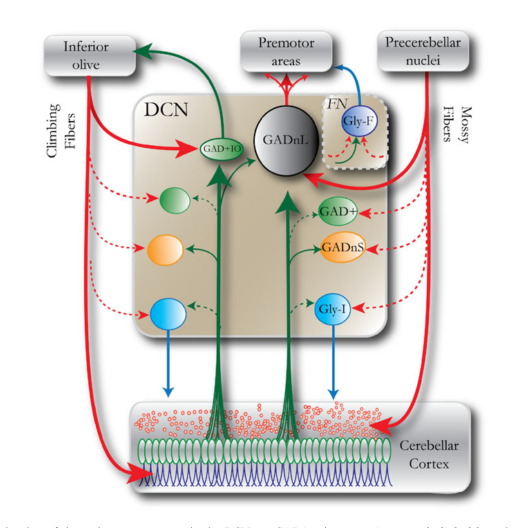
\includegraphics[scale=0.50]{images/uusisaari.png}
  \caption[GAD+IO neuron populations receive signals from cerebellar output]{GAD+IO neuron populations receive signals from cerebellar output \cite{Uusisaari2011}}
  \label{fig:uusisaari}
\end{figure}

\section{Experimental design and simulations}

\begin{figure}
  \centering
  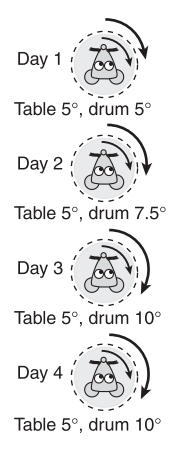
\includegraphics[scale=0.50]{images/vvor.png}
  \caption[VOR phase reversal adaptation protocol]{VOR phase reversal adaptation protocol as in \cite{Wulff2009a}}
  \label{fig:vvor}
\end{figure}

\begin{figure}
  \centering
  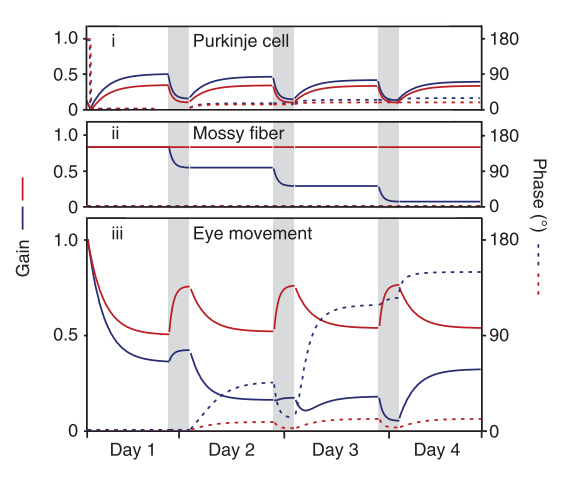
\includegraphics[scale=0.50]{images/gain.png}
  \caption[Wulff results on the VOR phase reversal adaptation protocol]{Wulff results on the VOR phase reversal adaptation protocol \cite{Wulff2009a}. Blue lines on the plots correspond to wild type mice behavior, that is what simulations of the model have to reproduce}
  \label{fig:wulffresults}
\end{figure}

Simulations of the VOR phase reversal adaptation protocol  (Figure \ref {fig:vvor}) have been made with Clopath's original model and with the NOI variation to reproduce experimental behavior in mice as in (Figure \ref {fig:wulffresults}).

\chapter{Results}

\section{Simulations an reproducibility}

Source code and reports of the simulations have been made available on a GitHub repository at http://xdurana.github.io/vor/ for reproducibility purposes.

\section{Nucleo-olivary inhibition model explains extinction}

Simulations of Clopath's detailed model (Figure \ref {fig:clopathgain}) and NOI model (Figure \ref {fig:longnoigain}) show that both are capable to adapt to different target gains after enough time on training sessions. Retinal slip, the error signal, is minimized after the training and the normalized gain is close to the target gain in both models.

The difference between the two models is at the behavior on the light deprivation pauses between training sessions. Clopath model learning on cerebellar cortex decays linearly without converging to an initial value or baseline, but NOI model makes cerebellar learning converge to a baseline exponentially. This behaviour is what's been shown experimentally.

\begin{figure}
  \centering
  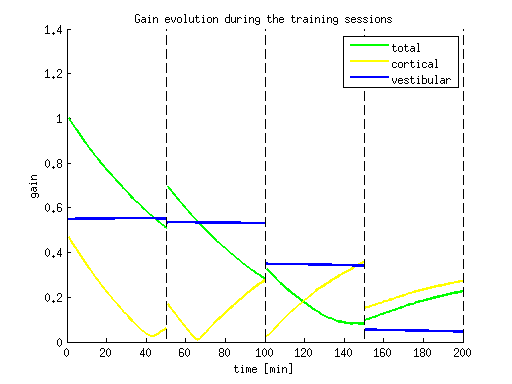
\includegraphics[scale=0.8]{images/clopath_11.png}
  \caption[Gain evolution on Clopath's model]{Gain evolution on Clopath's model}
  \label{fig:clopathgain}
\end{figure}

\begin{figure}
  \centering
  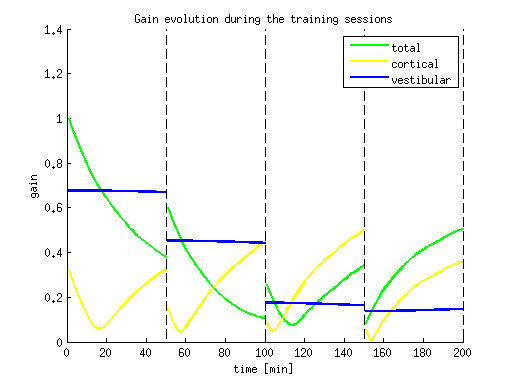
\includegraphics[scale=0.8]{images/longnoi_12.png}
  \caption[Gain evolution on the NOI model]{Gain evolution on the NOI model}
  \label{fig:longnoigain}
\end{figure}

\chapter{Discussion \& Conclusion}

\section{Complexity of the computational models of the VOR}

Computational models of the cerebellum have grown in complexity for the last decade due to the technical improvements on physiological measurements and experimental paradigms. This implies that every now and then bottom-up models have to be revised to include the findings and top-down or more functional models fail to describe the complexity of the circuitry.

\section{Relevance with respect to state of the art}

We have added the nucleo-olivary inhibition as an existing physiological connection on a state of the art computational model and we have shown that simulations reproduce more parsimoniously experimental behaviour on VOR adaptation. This extinction mechanism on VOR hasn't been modeled as NOI so far.

\section{Future steps}

To finally assess the validity of the results, the implementation of the model on closed-loop robotic simulations with the different adaptation paradigms would be necessary to determine the effectiveness of the model.

\begin{appendices}

\chapter{Appendix}

\section{Microcircuitry of the cerebellum}

The three-neuronal pathway formed by mossy fibers, granule cells and Purkinje cells conforms the substrate of the multilayered computational networks of the cerebellum. Mossy fibers and climbing fibers are the inputs, and Purkinje cells are the sole output of the cerebellar cortex. As Purkinje cells project to and inhibit their target neurons in the vestibular and deep cerebellar nuclei, the entire output of the cerebellum is inhibitory.

\begin{figure}
  \centering
  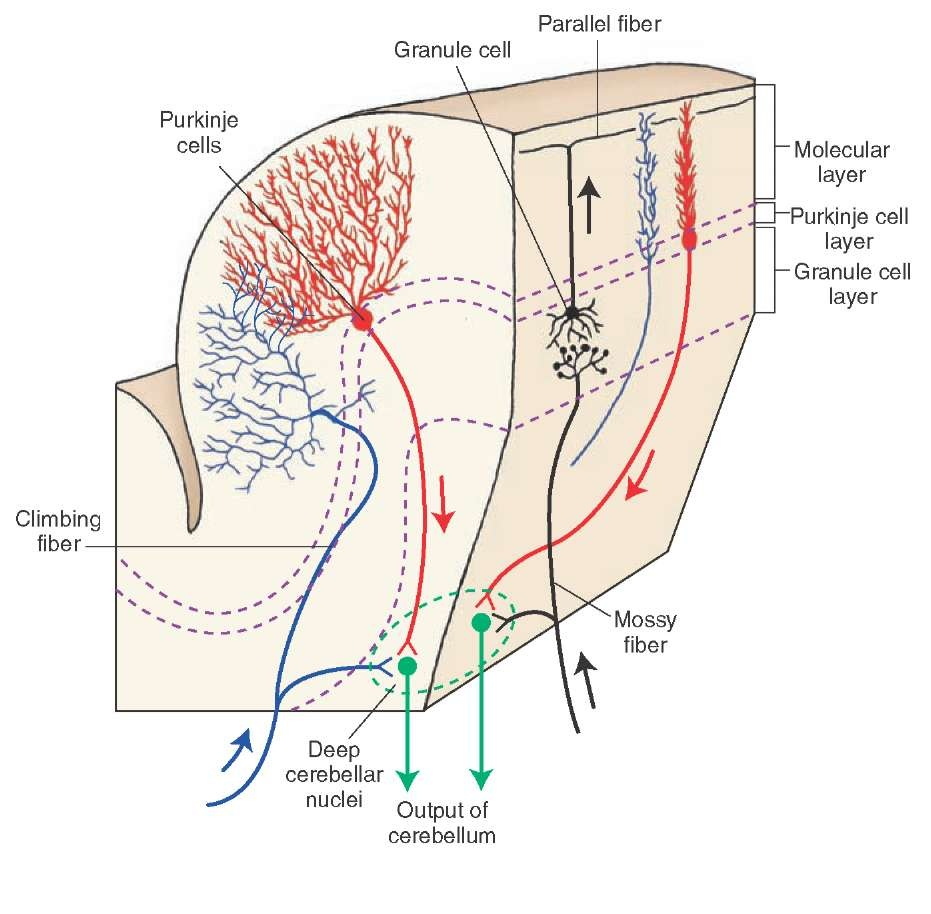
\includegraphics[scale=1]{images/circuit.jpg}
  \caption[Microcircuit of the cerebellum]{Microcircuit of the cerebellum}
\end{figure}

Mossy fibers convey information from different sources and synapse to 400 to 600 granule cells, that are the smallest and numerous neurons in the brain \cite{Marr1969}. On the contrary, granule cells integrates only a small number of mossy fibers conforming sparse coding \cite{Ito2006}. Granule cell axons bifurcate and form parallel fibers which run along the surface of the cerebellum.

Purkinje cells receive two very different types of input that have different electrophisiological effects. Parallel fibers synapse extensively on Purkinje cells and cause them to produce normal action potentials or simple spikes. Each Purkinje cell is also innervated by a single climbing fiber, arising from the inferior olive, that forms numerous synaptic contacts with the Purkinje cell dendrites. This is one of the most powerful synaptic junctions existing on the central nervous system, and every time climbing fibers fires the innervated Purkinje cell triggers a complex spike.

Parallel fibers also synapse to basket and stellate cells, the two types of interneurons of the molecular layer. They inhibit Purkinje cells and are contacted by climbing fibers. Because they are seldom differenced they are collectively called inhibitory interneurons \cite{Jorntell2010}.

\section{Marr-Albus classical models}

Different models have been developed on the last forty years to explain the role of the cerebellum on motor learning tasks, most of them deriving from the classical Marr-Albus theory \cite{Marr1969,Albus1971}. The idea of the theory arises from the observation that two very different signals affect indirectly the output of the cerebellum: thousands of weak inputs from parallel fibers are integrated on the Purkinje cell to generate simple spikes; and complex spikes are provoked by the strength of a single climbing fiber synapse. The basic concept is that learning involves plasticity at the parallel fiber to Purkinje cell synapses under control of the climbing fiber that provides an error or teaching signal as in classical supervised learning paradigms. The discovery of cerebellar long-term depression (LTD) of parallel fiber synapses onto Purkinje cells \cite{Ito1982} drove to a reinterpretation of the theory where LTD was the single plasticity mechanism of cerebellar learning.

In VOR adaptation, this teaching signal is assumed to be the retinal slip, that is the motion of the visual image on the surface of the retina. When images on the retina are still then retinal slip is silent and a signal that VOR is calibrated. On the contrary, when retinal slip is present the oculomotor plant has to be compensated. This faces us with the motor-error problem: VOR adaptation, as an feed-forward system has to send motor commands to the oculomotor plant to stabilize the image on the retina. But the perfect motor commands are not known, and the error signal that arrives at the cerebellum, the retinal slip, is sensory rather than motor information.

To solve the motor-error problem, Dean and Porril define a decorrelation rule that minimizes correlations between eye movements as a predictor variable and retinal slip as a target variable \cite{Dean2002}. The cerebellum receives information from the mossy fibers that is integrated onto Purkinje cells and decorrelated from the retinal slip. The output signal from the Purkinje cells is added to the vestibular information of the head movements to produce the new motor command. Depending whether the information conveyed by mossy fibers inputs to the cerebellum is vestibular or efferent copies of the motor commands, VOR adaptation forms a recurrent or a feedback architecture \cite{Porrill2004}.

\section{Adaptive filter models}

The idea that the cerebellum's role in adaptation could be understood in terms of control theory led to the theory of the cerebellum as an adaptive filter. The mossy fiber signal input is analyzed in granule cells, then weighted in parallel fibers and Purkinje cells (PF-PC) synapses and finally recombined to produce the output of the filter. The adaptation consists on the bidirectional adjustment of the weights on the PF-PC, that are reduced through LTD when the parallel fiber signal is correlated with the error, and are increased through long-term potentiation (LTP) when the correlation is negative \cite{Dean2010}.

One of the predictions of the adaptive filter model that are accomplished is that most PF-PC synapses are silent. This is coherent with the idea that most of the parallel fibers are carrying signals that are irrelevant to the specific learning task, and for that they are noise. Also, the decorrelation rule needs to be able to switch between positive or negative values of the weights but the synapses are either excitatory or inhibitory. This gap can be bridged if the inhibitory interneurons pathway from granule cells to Purkinje cells are considered.

The adaptive filter model shows accurate learning on VOR adaptation when the retinal slip is not delayed. The problem is that physiological experiments show that retinal slip error signal arrives at the flocculus with a delay of 100ms. The delay causes an impairment on learning on the model at frequencies up to 10Hz achieved with an eligibility trace, but humans can perform accurately up to 25Hz \cite{Porrill2007}. This questions that cortical plasticity may be not enough for VOR adaptation task.

\section{Plasticity on the brainstem}

The Miles-Lisberger was an alternative model where the role of the cerebellum was not to store the motor memory but rather to compute the instructive signal, carried by Purkinje cells, guiding the induction of plasticity in the vestibular nucleus \cite{Lac1995}.

For some time the two models could explain partially physiological observations of the experimentation until a growing body of evidence due to experimental improvements showed that additional sites of plasticity appear to contribute to motor adaptation \cite{Gao2012a}. Some VOR experiments with monkeys pointed to a site of synaptic plasticity not in cerebellar cortex but in the brainstem \cite{Lisberger2009a}, and consensus emerged that plasticity is required for VOR adaptation both at brainstem and cerebellar cortical sites. Other studies have reported motor learning in VOR adaptation task when eliminating the climbing fiber instructive signal, suggesting that both cortical and brainstem signals produce an additive effect when both are present but neither are indispensable for motor learning \cite{Ke2009a}.

There's a question whether learning starts on the cerebellar cortex or on the brainstem. It seems that cerebellar cortex starts learning early in VOR adaptation and progressively the gain learned is transfered to the brainstem. The task of the brainstem would be to learn a simple gain to keep the cerebellar cortex plasticity free for tasks that need a quicker adaptation.

%\chapter{Source code}
%\lstinputlisting[language=Matlab]{../simulations/parametric/VOR.m}

\end{appendices}

\bibliography{vor}

\backmatter
%\printindex

\end{document}


%NUMERACIÓ DE LA PÀGINA EXTERIOR EXCEPTE EN LA PRIMERA PÀGINA DE CADA CAPÍTOL
\usepackage{fancyhdr}
\pagestyle{fancy}
\fancyfoot{}
\fancyfoot[RO]{\thepage}
\fancyfoot[LE]{\thepage}


%MUTIPLES ÍNDEX
%En el preàmbul
%\usepackage{multind}
%\makeindex{authors}
%Introducció d'entrades la forma
%\index{authors}{Einstein}
%Situació de l'Índex
%\printindex{authors}{Author index}
%Cal eliminar les comandes \usepakage{makeidx} \makeindex \printindex
%cal exacutar des de la línia de comandes makeindex authors
